\documentclass[12pt,a4paper]{article}
\usepackage[utf8]{inputenc}
\usepackage[T1]{fontenc}
\usepackage{amsmath,amssymb}
\usepackage{geometry}
\usepackage{listings}
\usepackage{xcolor}
\usepackage{hyperref}
\usepackage{booktabs}
\usepackage{tikz}
\usetikzlibrary{arrows.meta,shapes,positioning}

\geometry{margin=2.5cm}
\lstset{
  basicstyle=\ttfamily\footnotesize,
  breaklines=true, frame=single,
  backgroundcolor=\color{gray!5},
  numbers=left, numberstyle=\tiny\color{gray}
}

\title{\textbf{Report 6: ROMFS Airframe, Parameters, and Flight Configuration}\\
\large Soaring Parameter Definitions and Default Airframe Setup\\[0.5em]
\normalsize PX4 Autosoaring Implementation --- Defence Technical Report}
\author{Radhouene --- Fixed-Wing Autosoaring Project}
\date{April 2026}

\begin{document}
\maketitle
\tableofcontents
\newpage

%=============================================================================
\section{ROMFS and Parameter Infrastructure}
%=============================================================================

\subsection{PX4 Parameter System}

PX4 parameters are persistent key-value pairs stored in:
\begin{itemize}
  \item \texttt{/fs/microsd/} (SD card on hardware, or simulated in SITL);
  \item compiled into the flash image with default values via
        \texttt{PARAM\_DEFINE\_*} macros in \texttt{.c} files.
\end{itemize}

Each parameter has:
\begin{itemize}
  \item a unique 16-character name;
  \item a type (\texttt{INT32}, \texttt{FLOAT});
  \item a default value;
  \item optional min/max and increment hints for GCS display.
\end{itemize}

\subsection{ROMFS Airframe Files}

The \texttt{ROMFS/px4fmu\_common/init.d/airframes/} directory contains
shell scripts that run at boot. They set parameters for a specific vehicle
configuration. The airframe file referenced in this project is:

\begin{lstlisting}
ROMFS/px4fmu_common/init.d/airframes/4008_gz_advanced_plane
\end{lstlisting}

This is a Gazebo SITL airframe for a generic advanced plane used during
development and simulation.

%=============================================================================
\section{Parameter Definitions in fw\_path\_navigation\_params.c}
%=============================================================================

\subsection{Original Parameters (Powered-Only)}

In the original codebase, the fixed-wing navigation parameters file
contained no soaring-specific entries. The nearest relevant parameter was
a general airspeed parameter hierarchy:

\begin{itemize}
  \item \texttt{FW\_AIRSPD\_MIN} -- minimum EAS (stall margin) [m/s]
  \item \texttt{FW\_AIRSPD\_TRIM} -- cruise trim EAS [m/s]
  \item \texttt{FW\_AIRSPD\_MAX} -- maximum EAS [m/s]
\end{itemize}

\subsection{Removed Parameter: FW\_GLIDE\_MODE}

In the first implementation, a parameter \texttt{FW\_GLIDE\_MODE} was
defined as an integer to select between fixed-EAS glide (0) and polar
best-glide (1). This was removed in the redesign because the distinction
is now captured directly in \texttt{soaring\_mode}:

\begin{center}
\begin{tabular}{lll}
\toprule
Old \texttt{FW\_GLIDE\_MODE} & New \texttt{soaring\_mode} & Meaning \\
\midrule
0 & 1 (\texttt{SOARING\_GLIDE\_FIXED}) & Fixed EAS \\
1 & 2 (\texttt{SOARING\_GLIDE\_POLAR}) & Polar best-glide \\
\bottomrule
\end{tabular}
\end{center}

\subsection{New Soaring Parameters}

\subsubsection{FW\_GLIDE\_AIRSPD}

\begin{lstlisting}[language=C]
PARAM_DEFINE_FLOAT(FW_GLIDE_AIRSPD, 10.0f);
\end{lstlisting}

\textbf{Unit:} m/s (EAS) \\
\textbf{Range:} [5.0, 30.0] \\
\textbf{Purpose:} The fixed-EAS glide setpoint for mode 1. Also used as
the airspeed reference during thermalling (modes 3 and 4).

The parameter value is an \emph{Equivalent Airspeed (EAS)}, not TAS.
TECS performs the conversion:
\begin{equation}
  V_{\text{TAS}}^* = k_{\text{EAS2TAS}} \cdot V_{\text{EAS}}^*
  = \sqrt{\frac{\rho_0}{\rho}} \cdot V_{\text{EAS}}^*
\end{equation}

\textbf{Rationale for default 10.0 m/s:} A typical mini-UAV has a stall
speed around 8--9 m/s EAS. A 10 m/s glide speed provides a safe margin
above stall while keeping the glide angle shallow (small $\gamma = -w_s/V$).

\subsubsection{FW\_POLAR\_A}

\begin{lstlisting}[language=C]
PARAM_DEFINE_FLOAT(FW_POLAR_A, 0.003f);
\end{lstlisting}

\textbf{Unit:} s/m \\
\textbf{Description:} Quadratic coefficient $a$ of the glide polar:
\begin{equation}
  w_s(V) = a V^2 + b
\end{equation}

\textbf{Physics:} $a$ scales with induced drag. Its value is:
\begin{equation}
  a = \frac{k}{\pi e AR \frac{1}{2}\rho S V^2 / (mg)} 
  = \frac{2(mg)k}{\pi e AR \rho S}
\end{equation}
(approximate form). For a $2\,\text{kg}$, $0.8\,\text{m}^2$ wing, span
$2\,\text{m}$: $a \approx 0.003$.

\subsubsection{FW\_POLAR\_B}

\begin{lstlisting}[language=C]
PARAM_DEFINE_FLOAT(FW_POLAR_B, 0.5f);
\end{lstlisting}

\textbf{Unit:} m/s \\
\textbf{Description:} Constant term $b$ of the glide polar (minimum sink rate).

\textbf{Physics:} $b$ corresponds to parasitic drag at very low speed:
\begin{equation}
  b \approx \frac{W}{T_{\max}}\,w_{s,0}
\end{equation}

For a $2\,\text{kg}$ aircraft with $V_{\text{min-sink}} \approx 0.5\,\text{m/s}$:
$b = 0.5$.

\subsubsection{Best-Glide Derivation from A and B}

\begin{equation}
  \boxed{
    V^*_{\text{EAS,polar}} = \sqrt{\frac{b}{a}} = \sqrt{\frac{0.5}{0.003}} \approx 12.9\,\text{m/s}
  }
\end{equation}

The glide ratio at this speed:
\begin{equation}
  \frac{L}{D}\bigg|_{\text{max}} = \frac{V^*}{w_s(V^*)}
  = \frac{\sqrt{b/a}}{a(b/a) + b}
  = \frac{1}{2\sqrt{ab}}
  = \frac{1}{2\sqrt{0.003 \times 0.5}} = \frac{1}{0.0775} \approx 12.9
\end{equation}

\subsubsection{FW\_GLIDE\_I\_DECAY}

\begin{lstlisting}[language=C]
PARAM_DEFINE_FLOAT(FW_GLIDE_I_DECAY, 10.0f);
\end{lstlisting}

\textbf{Unit:} s \\
\textbf{Description:} Throttle integrator decay time constant $\tau$ during
gliding:
\begin{equation}
  I_t(t) = I_t(0)\,e^{-t/\tau}
\end{equation}

After $3\tau = 30\,\text{s}$, the integrator retains only $e^{-3} \approx 5\%$
of its pre-glide value.

\subsubsection{FW\_GLIDE\_RAMP\_T}

\begin{lstlisting}[language=C]
PARAM_DEFINE_FLOAT(FW_GLIDE_RAMP_T, 3.0f);
\end{lstlisting}

\textbf{Unit:} s \\
\textbf{Description:} Duration of the symmetric entry/exit throttle ramps.

\textbf{Sizing:} A $3\,\text{s}$ ramp at $50\,\text{Hz}$ corresponds to
150 control cycles. With $\Delta\delta_t = 0.4$ (typical cruise throttle),
the rate is $0.133\,\text{per second}$.

\subsubsection{FW\_THERMAL\_BANK}

\begin{lstlisting}[language=C]
PARAM_DEFINE_FLOAT(FW_THERMAL_BANK, 40.0f);
\end{lstlisting}

\textbf{Unit:} degrees \\
\textbf{Description:} Default bank angle for thermalling when the companion
does not specify \texttt{bank\_angle\_cmd}.

\textbf{Physics:} At $\phi = 40^\circ$, the load factor and turn radius are:
\begin{align}
  n_z &= 1/\cos(40^\circ) = 1.305 \\
  R_{\min} &= \frac{V^2}{g\tan\phi}
            = \frac{10^2}{9.81 \times \tan(40^\circ)} \approx 12.2\,\text{m}
\end{align}

\subsubsection{FW\_ALT\_MIN and FW\_ALT\_MAX}

\begin{lstlisting}[language=C]
PARAM_DEFINE_FLOAT(FW_ALT_MIN,  50.0f);
PARAM_DEFINE_FLOAT(FW_ALT_MAX, 200.0f);
PARAM_DEFINE_FLOAT(FW_ALT_HYST, 20.0f);
\end{lstlisting}

Safety altitude bounds:
\begin{itemize}
  \item \texttt{FW\_ALT\_MIN}: soaring inhibited below this AGL altitude.
  \item \texttt{FW\_ALT\_MAX}: thermal mode forced off above this altitude.
  \item \texttt{FW\_ALT\_HYST}: hysteresis on the ceiling to prevent chatter.
\end{itemize}

%=============================================================================
\section{ROMFS Airframe: 4008\_gz\_advanced\_plane}
%=============================================================================

\subsection{Purpose}

The ROMFS airframe script sets default parameter values for the Gazebo
SITL ``advanced plane'' model. Changes were made to add soaring defaults.

\subsection{Added Parameter Defaults}

\begin{lstlisting}[language=bash]
# Autosoaring parameters
param set FW_GLIDE_AIRSPD   10.0
param set FW_POLAR_A         0.003
param set FW_POLAR_B         0.5
param set FW_GLIDE_I_DECAY  10.0
param set FW_GLIDE_RAMP_T    3.0
param set FW_THERMAL_BANK   40.0
param set FW_ALT_MIN        50.0
param set FW_ALT_MAX       200.0
param set FW_ALT_HYST       20.0
\end{lstlisting}

\subsection{Justification for Default Values}

\begin{center}
\begin{tabular}{lccl}
\toprule
Parameter & Value & Unit & Rationale \\
\midrule
\texttt{FW\_GLIDE\_AIRSPD}  & 10.0 & m/s EAS & $\sim 25\%$ above stall \\
\texttt{FW\_POLAR\_A}        & 0.003 & s/m   & Typical mini-UAV induced drag \\
\texttt{FW\_POLAR\_B}        & 0.5 & m/s     & Typical mini-UAV parasitic drag \\
\texttt{FW\_GLIDE\_I\_DECAY} & 10 & s        & 5\% residual after 30 s \\
\texttt{FW\_GLIDE\_RAMP\_T}  & 3 & s         & 150 cycles at 50 Hz \\
\texttt{FW\_THERMAL\_BANK}   & 40 & deg       & $R_{\min}=12.2\,\text{m}$ at 10 m/s \\
\texttt{FW\_ALT\_MIN}        & 50 & m AGL     & Terrain clearance \\
\texttt{FW\_ALT\_MAX}        & 200 & m AGL    & Typical soaring ceiling \\
\texttt{FW\_ALT\_HYST}       & 20 & m         & $\sim 10\%$ of ceiling range \\
\bottomrule
\end{tabular}
\end{center}

%=============================================================================
\section{Complete Parameter Dependency Graph}
%=============================================================================

The following shows how each parameter flows into the control pipeline:

\begin{center}
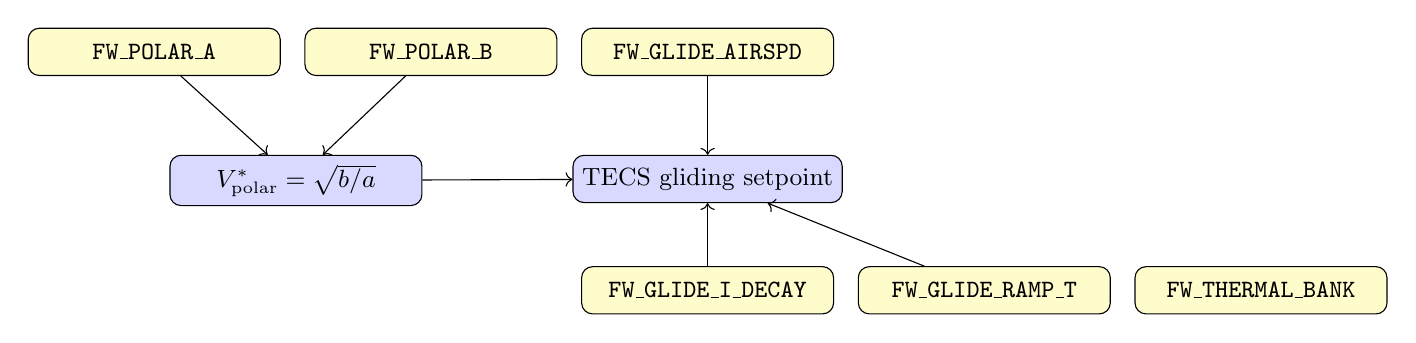
\begin{tikzpicture}[node distance=1.4cm,
    param/.style={draw,fill=yellow!20,rounded corners,minimum width=3.2cm,minimum height=0.6cm,align=center,font=\small},
    mod/.style={draw,fill=blue!15,rounded corners,minimum width=3.2cm,minimum height=0.6cm,align=center,font=\small}]
  \node[param] (a) {\texttt{FW\_POLAR\_A}};
  \node[param,right=0.3cm of a] (b) {\texttt{FW\_POLAR\_B}};
  \node[mod,below=1cm of a, xshift=1.8cm] (polar) {$V^*_{\text{polar}} = \sqrt{b/a}$};
  \node[param,right=0.3cm of b] (airspd) {\texttt{FW\_GLIDE\_AIRSPD}};
  \node[mod,below=1cm of airspd] (tecs) {TECS gliding setpoint};
  \node[param,below=0.8cm of tecs] (idecay) {\texttt{FW\_GLIDE\_I\_DECAY}};
  \node[param,right=0.3cm of idecay] (ramp) {\texttt{FW\_GLIDE\_RAMP\_T}};
  \node[param,right=0.3cm of ramp] (bank) {\texttt{FW\_THERMAL\_BANK}};
  \draw[->] (a) -- (polar);
  \draw[->] (b) -- (polar);
  \draw[->] (polar) -- (tecs);
  \draw[->] (airspd) -- (tecs);
  \draw[->] (idecay) -- (tecs);
  \draw[->] (ramp) -- (tecs);
\end{tikzpicture}
\end{center}

%=============================================================================
\section{Summary}
%=============================================================================

\begin{center}
\begin{tabular}{p{4.5cm}p{4.5cm}p{4.5cm}}
\toprule
Aspect & Original & Modified \\
\midrule
Soaring parameters & None & 9 new parameters \\
FW\_GLIDE\_MODE & Defined (integer, polar select) & Removed (mode in message) \\
Airframe defaults & No soaring values & Added to \texttt{4008\_gz\_advanced\_plane} \\
Polar model & Not present & $w_s = aV^2 + b$ with $a$, $b$ params \\
\bottomrule
\end{tabular}
\end{center}

\end{document}
